\chapter{Конструкторский раздел}

В данном разделе формализуются сущности системы, определяется ролевая модель и выбираются необходимые процедуры/функции/триггеры. Каждой сущности, описанной в аналитическом разделе соотносятся поля --- информация, необходимая для полного их определения. На основе этой информации создаётся ER-диаграмма базы данных, в которой указываются все таблицы необходимы для правильной работы системы. Также создаётся схема триггера, используемого в системе.

\section{Описание сущностей}

В предыдущем разделе были сформулированы сущности разрабатываемой базы данных. Далее приведён полный набор полей каждой сущности.
\begin{enumerate}[label=\arabic*.]
	\item \textbf{Owner} --- таблица владельцев словарей;
	\begin{enumerate}[label=\alph*.]
		\item id --- порядковый номер владельца, число, первичный ключ;
		\item name --- имя владельца, строка;
		\item age --- дата рождения владельца, дата;
		\item disease --- отклонение владельца, строка;
	\end{enumerate}
	\item \textbf{Noun} --- главные слова;
	\begin{enumerate}[label=\alph*.]
		\item id --- порядковый номер слова, число, первичный ключ;
		\item ownerid --- порядковый номер владельца, число, внешний ключ;
		\item word --- само слово, строка;
		\item picture --- картинка PECS, фотография;
		\item record --- запись произношения слова, звуковой файл;
	\end{enumerate}
	\item \textbf{SubAction} --- действия термина как субъекта;
	\begin{enumerate}[label=\alph*.]
		\item id --- порядковый номер слова, число, первичный ключ;
		\item word --- само слово, строка;
		\item picture --- картинка PECS, фотография;
		\item record --- запись произношения слова, звуковой файл;
	\end{enumerate}
	\item \textbf{ObAction} --- действие термина как объекта;
	\begin{enumerate}[label=\alph*.]
		\item id --- порядковый номер слова, число, первичный ключ;
		\item word --- само слово, строка;
		\item picture --- картинка PECS, фотография;
		\item record --- запись произношения слова, звуковой файл;
	\end{enumerate}
	\item \textbf{Adjective} --- характеристики слов;
	\begin{enumerate}[label=\alph*.]
		\item id --- порядковый номер слова, число, первичный ключ;
		\item word --- само слово, строка;
		\item picture --- картинка PECS, фотография;
		\item record --- запись произношения слова, звуковой файл.
	\end{enumerate}
\end{enumerate}

На рисунке \ref{DB} представлена ER-диаграмма базы данных.
\begin{figure}[ht!]\centering
	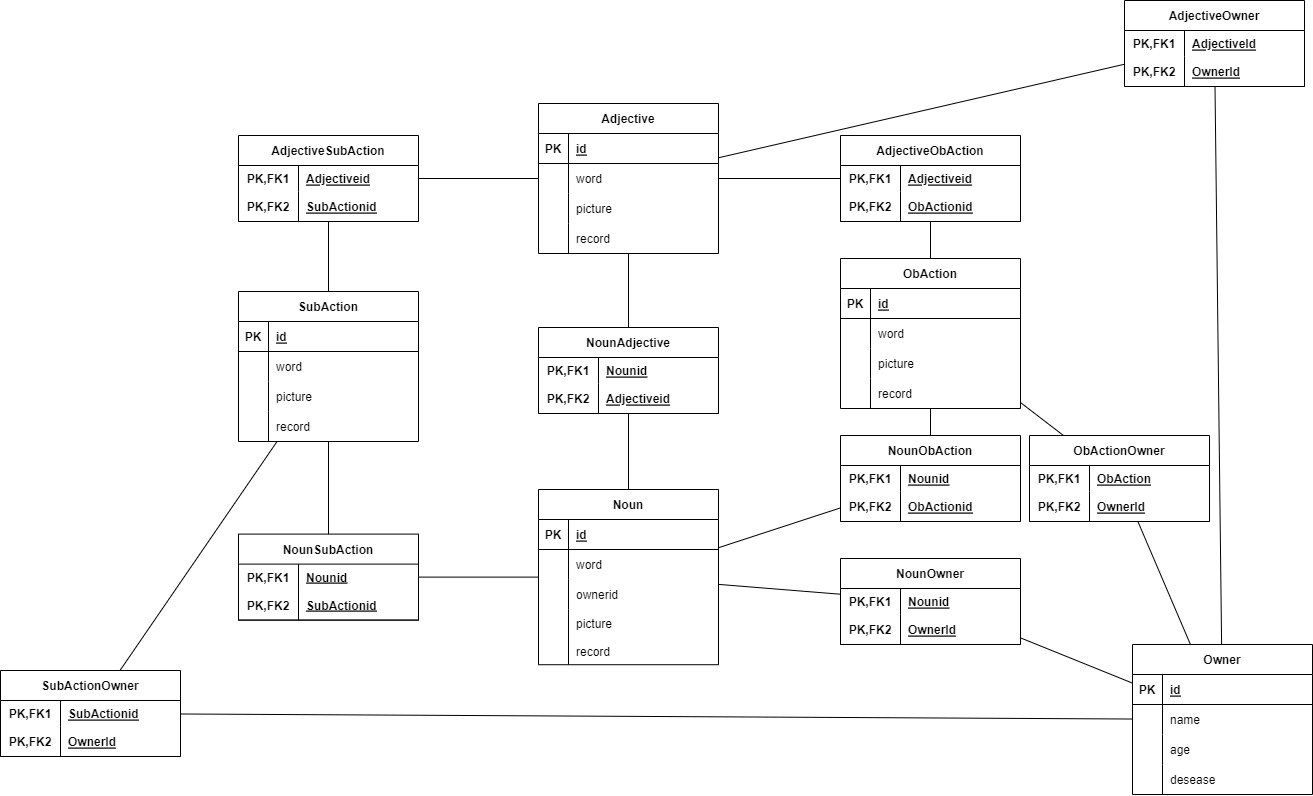
\includegraphics[scale=0.35]{ER}
	\caption{ER-диаграмма базы данных}
	\label{DB}
\end{figure}

\section{Ролевая модель}

Ролевая модель в системе необходима для того, чтобы правильно организовать работу пользователей в системе, предоставляя каждому пользователю определённый набор действий в системе.

Для работы пользователей с базой данных выделяется следующая ролевая модель:
\begin{enumerate}[label=\arabic*.]
	\item doctor --- психолог. Имеет все права над всеми таблицами;
	\item patient --- пациент. Имеет доступ SELECT ко всем таблицам.
	\item family --- родственник. Имеет доступ SELECT и UPDATE ко всем таблицам.
\end{enumerate}

\section{Используемые триггеры}

В системе представлен триггер, позволяющий удалять все узлы, оказавшиеся без единой связи с сущностью <<Владелец>>, после удаления очередного узла из БД.

На рисунке \ref{trigger} представлена схема триггера.

\begin{figure}[ht!]\centering
	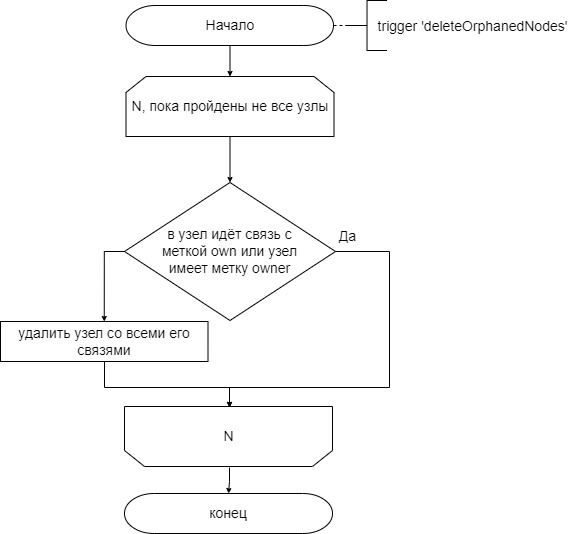
\includegraphics[scale=0.5]{trigger}
	\caption{Схема триггера}
	\label{trigger}
\end{figure}


\section*{Вывод}

В данном разделе были целиком описаны сущности системы, представлена ER-диаграмма базы данных, выбрана ролевая модель. Описаны используемые процедуры/функции/триггеры.